\documentclass[tikz,border=10pt]{standalone}
\usepackage{tikz}
\usetikzlibrary{arrows.meta,positioning}

\tikzset{
  card/.style={draw=blue!70!black, line width=1.2pt, rounded corners=3pt, minimum width=5.6cm, minimum height=1.0cm, align=center, fill=none},
  note/.style={draw=orange!80!black, line width=1.2pt, rounded corners=3pt, minimum width=5.6cm, minimum height=1.0cm, align=center, fill=none},
  flow/.style={-{Stealth[length=3mm]}, line width=1.2pt, draw=black!70}
}

\begin{document}
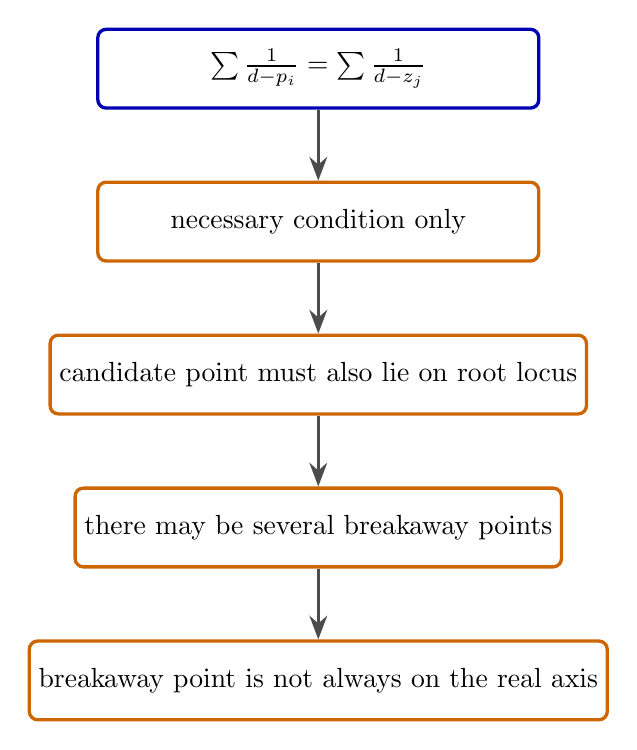
\begin{tikzpicture}[node distance=0.9cm]
  \node[card] (a) {$\sum \frac{1}{d-p_i}=\sum \frac{1}{d-z_j}$};
  \node[note, below=of a] (b) {necessary condition only};
  \node[note, below=of b] (c) {candidate point must also lie on root locus};
  \node[note, below=of c] (d) {there may be several breakaway points};
  \node[note, below=of d] (e) {breakaway point is not always on the real axis};

  \draw[flow] (a) -- (b);
  \draw[flow] (b) -- (c);
  \draw[flow] (c) -- (d);
  \draw[flow] (d) -- (e);
\end{tikzpicture}
\end{document}
